\section{Extensions of $\R$: the Complex Numbers \C}

\begin{definition}
	\emph{The Extended Reals}: $\overline{\R}:=\{-\infty ,\infty\}\cup \R$ , with the usual order on $\R$, with $-\infty <x<\infty$, for all $x\in\R$, such that: 
    
    \begin{enumerate}
	    \item $x\pm \infty = \pm \infty$
        \item $x\cdot\infty = \pm\infty$
        \item $\frac{x}{\infty}=0$


	\end{enumerate}
    And so forth.
    \end{definition}
    
This set shares many features with the real numbers, but it is important to note that it itself is not an ordered field. The reason that we care about the extended reals, then, is that \emph{every $A\subset \overline{\R}$ has a supremum.}

\begin{definition}
	\emph{Euclidean Space:} $\R^k := \{(x_1,x_2,...,x_n):x_i \in \R\}$, such that $(x_1,...,x_n)+(y_1,...,y_n)=(x_1+y_1,...,x_n+y_n)$.  
\end{definition}

This set also is often useful, despite not being an ordered field. A special case of Euclidean space is the vector space, which we develop in the following:

\begin{definition} \emph{Vector Space Properties}:
	\begin{enumerate}
	    \item \emph{Scalar Multiplication}: $\alpha(x_1,...,x_n)=\alpha\mathbf{x}=(\alpha x_1, ..., \alpha x_n)$
        \item \emph{Dot Product}: $\mathbf{x} \cdot \mathbf{y} = \sum ^k_i x_iy_i$
        \item \emph{Norms}: $|\mathbf{x}|:=\sqrt{x_1 + ... + x_n}$
	\end{enumerate}
  
\end{definition}
\begin{figure}
    \centering
    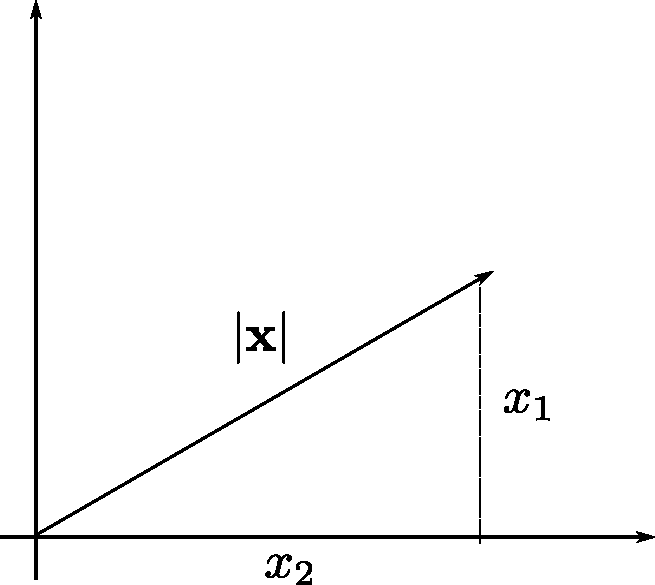
\includegraphics[width=0.4\linewidth]{figures/norm.pdf}
    \caption{A 2-tuple in Euclidean 2-space represented on the plane.}
    \label{fig:enter-label}
\end{figure}



One can see that the concept of a norm is analogous to that of Euclidean distance, with the norm acting as a generalization of the Pythagorean theorem.

\begin{definition}
    \emph{The Complex Number Field $\C$}: For $(a,b)\in \R^2$, let: \begin{enumerate}
        \item $(a,b)+(c,d) = (a+b ,  c+d)$
        \item $(a,b)\cdot (c,d) = (ac-bd,ad+bc)$
        \item $(0,0)$ and $(1,0)$ are the additive and multiplicative identities, respectively
        \item $(0,1)=i$
        \item For $z=a+bi\in \C$, $\overline{z}=a-bi$
        \end{enumerate}
\end{definition}

$\C$ is a natural extension of $\R$ (i.e., $\{a+0i:a\in \R\}$ is isomorphic to $\R^2$). Note: $(0,1)\cdot(0,1)=(-1,0)$, so $i^2 = -1$.

\begin{figure}[H]
        \centering
        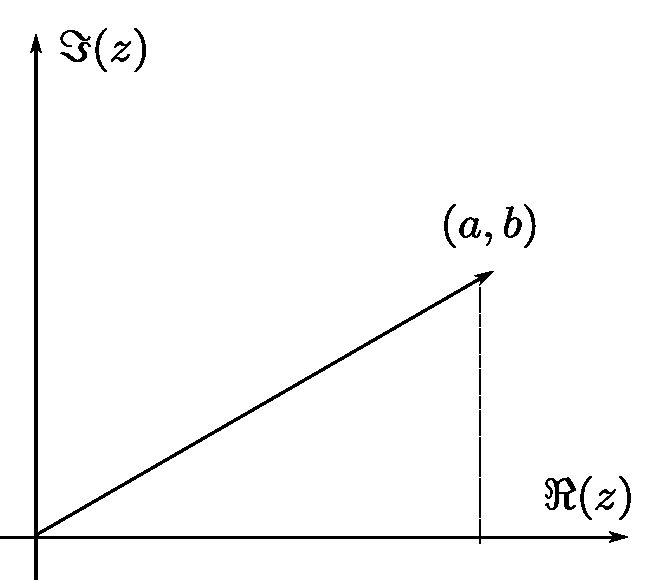
\includegraphics[width=0.4\linewidth]{figures/imag(ab)plane.pdf}}
        \caption{A planar representation of $z=(a,b)\in \C$.}
        \label{fig:enter-label}
    \end{figure}

\begin{theorem}
	\emph{The Cauchy-Shawrz Inequality}: If $a_1,...,a_n$ and $b_1,...,b_n$ are complex numbers, then $$\left|\sum^n_{i=0} a_i\overline{b_i}\right|^2 \leq \sum^n_{i=0}|a_i|^2 \cdot \sum^n_{i=0}|b_i|^2$$ will hold.
\end{theorem}